\documentclass[12pt,aspectratio=169]{beamer}
\usepackage{
  amsfonts,amsmath,amssymb,
  derivative,
  epigraph,
  geometry,
  isomath,
  listings,
  mathtools,
  parskip,
  tikz
}
\usepackage[framed,numbered]{matlab-prettifier}
\usepackage{algorithmic,algorithm}
\usepackage[backend=bibtex,style=authoryear]{biblatex}
\addbibresource{../na_refs.bib}
\usepackage{hyperref}
\usetikzlibrary{arrows.meta,calc,shapes.geometric,positioning}
\tikzset {
  >=Stealth,
  every node/.style={font=\small},
}

\hypersetup{
  colorlinks=true,
  allcolors=ujorange
}

\usetheme{Hoepoe}
\usefonttheme[onlymath]{serif}
\beamertemplatenavigationsymbolsempty
\setbeamertemplate{footline}[frame number]
\AtBeginSection[]{
  \begin{frame}
  \vfill
  \centering
  \begin{beamercolorbox}[sep=8pt,center,shadow=true,rounded=true]{title}
    \usebeamerfont{title}\insertsectionhead\par%
  \end{beamercolorbox}
  \vfill
  \end{frame}
}

\def\modulecode{APM02B2}
\def\modulename{Introduction to Numerical Analysis}
%\def\topicno{00}
\def\topicname{Fixed Point Iteration}
\title{\modulecode\ \modulename}
\subtitle{\topicname}
\title[\modulecode]{\modulecode\ \modulename}
\author[Dr Anderson]{Dr K. D. Anderson}
\institute[UJ]{University of Johannesburg}
\def\logo{\includegraphics[width=100px]{../../img/UJ_logo.png}}
\titlegraphic{\logo}
\date{}

\renewcommand{\vec}{\vectorsym}
\providecommand{\mat}{\matrixsym}
\DeclarePairedDelimiter{\abs}{\lvert}{\rvert}
\DeclarePairedDelimiter{\norm}{\lVert}{\rVert}
\providecommand{\defeq}{\coloneqq}

\begin{document}
\frame{\maketitle}
\frame{%
  \tableofcontents 
  \epigraph{
    It is better to do the right problem the wrong way than the wrong problem
    the right way.
  }{\textit{Richard W. Hamming}}
}
%\begin{frame}
%  \begin{columns}[onlytextwidth]
%    \begin{column}{.45\textwidth}
%      \tableofcontents
%    \end{column}
%    \begin{column}{.45\textwidth}
%      \begin{quote}
%        ``The purpose of computing is insight, not
%        numbers.'' - \textit{Richard W. Hamming}
%      \end{quote}
%    \end{column}
%  \end{columns}
%\end{frame}

%\section{Introduction}
%\begin{frame}{Introduction}
%  Equations of various kinds arise in a range of applications.
%
%  Some equations are simple and easy to solve.
%
%  Consider, for example, the \emph{linear equation}
%  \begin{equation} \label{eq:linear-eq}
%    ax + b = 0,
%  \end{equation}
%  which has the solution
%  \begin{equation} \label{eq:linear-eq-soln}
%    x^* = -\frac{b}{a}, \quad
%    a \neq 0.
%  \end{equation}
%\end{frame}
%
%\begin{frame}{Introduction}
%  Some equations are \emph{nonlinear}.
%
%  The simplest example of a nonlinear equation is the \emph{quadratic equation}
%  \begin{equation} \label{eq:quadratic-eq}
%    ax^2 + bx + c = 0,
%  \end{equation}
%  which has the solution
%  \begin{equation} \label{eq:quadratic-eq-soln}
%    x^*_1 = \frac{-b + \sqrt{b^2 - 4ac}}{2a}, \quad
%    x^*_2 = \frac{-b - \sqrt{b^2 - 4ac}}{2a}, \quad
%    a \neq 0.
%  \end{equation}
%\end{frame}

\section{Problem Statement}
\begin{frame}{Problem Statement}
  Let $I \subset \mathbb{R}$ and $f : I \to \mathbb{R}$ be continuous on $I$.

  Generally, we assume that $I$ is a bounded and closed interval.
  That is,
  \[
    I = [a, b],
  \] 
  where $a, b \in \mathbb{R}$ such that $a < b$ (this
  guarantees that $I$ is not empty).

  \begin{block}{Problem}
  Consider the general equation
  \begin{equation} \label{eq:root-eq}
    f(x) = 0.
  \end{equation}
  We wish to find all $x^* \in I$ that satisfy equation \eqref{eq:root-eq}.
  These $x^*$ are called the \emph{roots of the function $f$}.
  \end{block}
\end{frame}

\section{Fixed Point Theory}
\begin{frame}{Fixed Points}
  An equivalent manner to solve \eqref{eq:root-eq} is by rewriting it in the
  form
  \begin{equation} \label{eq:fp-eq}
    x = g(x),
  \end{equation}
  where $g : [a,b] \to \mathbb{R}$ is a continuous function on $[a,b]$
  satisfying certain properties (which we shall discuss).

  Equation \eqref{eq:fp-eq} is referred to as a \emph{fixed-point equation}.
  \begin{definition}[Fixed point of a function]
    The solution $x^*$ to equation \eqref{eq:fp-eq} is called a \emph{fixed
    point of $g$}.
    That is, it is a number $x^*$ satisfying $x^* = g(x^*)$.
  \end{definition}
  \vskip -.5em
  A fixed point for a function is a number at which the value of the function
  does not change when the function is applied.
\end{frame}

\begin{frame}{Fixed Points}{Visualisation}
  We can visualise \textcolor{green!70!black}{fixed points} as the intersections
  of the graphs ${\color{red} y = g(x)}$ and ${\color{blue} y = x}$.
  \vskip \baselineskip
  \begin{columns}[onlytextwidth]
    \begin{column}{.45\textwidth}
      \begin{center}
        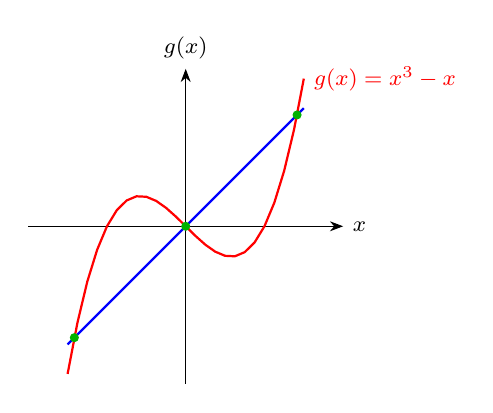
\begin{tikzpicture}[every node/.style={font=\footnotesize}]
          \draw[->] (-2,0) -- (2,0) node[right]{$x$};
          \draw[->] (0,-2) -- (0,2) node[above]{$g(x)$};
          \draw[blue,thick,domain=-3/2:3/2] plot(\x, \x);
          \draw[red,thick,domain=-3/2:3/2] plot(\x, {\x^3 - \x})
          node[right]{$g(x) = x^3 - x$};
          \filldraw[green!70!black] ({-sqrt(2)},{-sqrt(2)}) circle[radius=.5mm];
          \filldraw[green!70!black] (0,0) circle[radius=.5mm];
          \filldraw[green!70!black] ({sqrt(2)},{sqrt(2)}) circle[radius=.5mm];
        \end{tikzpicture}
      \end{center}
    \end{column}
    \begin{column}{.45\textwidth}
      \begin{center}
        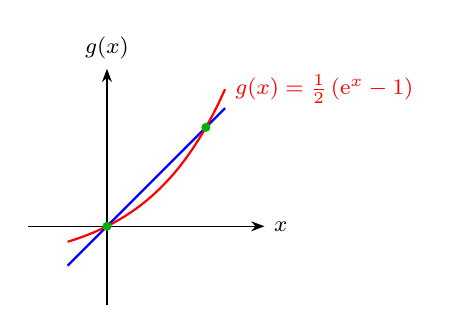
\begin{tikzpicture}[every node/.style={font=\footnotesize}]
          \draw[->] (-1,0) -- (2,0) node[right]{$x$};
          \draw[->] (0,-1) -- (0,2) node[above]{$g(x)$};
          \draw[blue,thick,domain=-1/2:3/2] plot(\x, \x);
          \draw[red,thick,domain=-1/2:3/2] plot(\x, {(exp(\x) - 1)/2})
          node[right]{$g(x) = \frac{1}{2}\left(\mathrm{e}^x - 1\right)$};
          \filldraw[green!70!black] (0,0) circle[radius=.5mm];
          \filldraw[green!70!black] (1.256431,1.256431) circle[radius=.5mm];
        \end{tikzpicture}
      \end{center}
    \end{column}
  \end{columns}
\end{frame}

\begin{frame}{Fixed Points}{Finding fixed points}
  \begin{example}
    Find the fixed point(s) of the function $g(x) = x^3 - x$.
  \end{example}
  Substituting the given function into the fixed-point equation \eqref{eq:fp-eq}
  yields the equation
  \[
    x = x^3 - x,
  \]
  which we solve for $x$:
  \[
    x = x^3 - x
    \quad \implies \quad
    0 = x^3 - 2x = x(x^2 - 2)
    \quad \implies \quad
    x^* = 0,\ x^* = \pm\sqrt{2}.
  \]
\end{frame}

\begin{frame}{Fixed Points}{Finding fixed points}
  If $g$ is a polynomial of degree $< 5$, we could find the fixed
  points algebraically via factorisation or long division.

  However, if $g$ is a polynomial of degree $\geq 5$, or a nonlinear function,
  we would need to resort to approximating the fixed points (see slide
  \ref{fr:fp-iter-def}).

  A lot can still be said about the fixed points themselves without solving
  equation \eqref{eq:fp-eq} by considering the properties of the function $g$.
\end{frame}


\begin{frame}{Fixed Points}{Existence and uniqueness}
  A function may have none, one, or many fixed points.

  The following questions now arise: 
  \begin{itemize}
    \item \textcolor{red}{%
      Under which circumstances do fixed points exist for a given
      function $g$?
      }
    \item \textcolor{red}{%
      What conditions must $g$ satisfy for a fixed point to be unique?
      }
  \end{itemize}
\end{frame}

\begin{frame}{Fixed Points}{Existence and uniqueness}
  \begin{columns}[onlytextwidth]
    \begin{column}{.45\textwidth}
      \begin{center}
        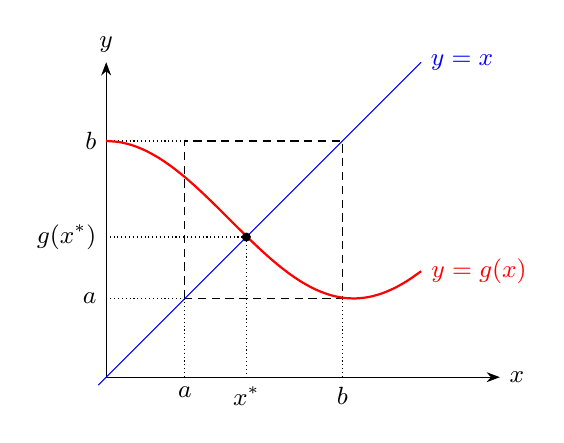
\begin{tikzpicture}
          \coordinate (a) at (1,1);
          \coordinate (ax) at (1,0);
          \coordinate (ay) at (0,1);
          \coordinate (b) at (3,3);
          \coordinate (bx) at (3,0);
          \coordinate (by) at (0,3);
          \coordinate (p) at (1.78,1.78);
          \coordinate (px) at (1.78,0);
          \coordinate (py) at (0,1.78);

          \draw[densely dashed] (a) -- (1,3) -- (b) -- (3,1) -- cycle;
          \begin{scope}[densely dotted]
            \draw (a) -- (ax) node[below]{$a$};
            \draw (3,1) -- (bx) node[below]{$b$};
            \draw (a) -- (ay) node[left]{$a$};
            \draw (1,3) -- (by) node[left]{$b$};
            \draw (p) -- (px) node[below]{$x^*$};
            \draw (p) -- (py) node[left]{$g(x^*)$};
          \end{scope}

          \draw[->] (0,0) -- (5,0) node[right]{$x$};
          \draw[->] (0,0) -- (0,4) node[above]{$y$};

          \draw[blue] (-1/10,-1/10) -- (4,4)node[right]{$y = x$};
          %\draw[red,thick,smooth] plot coordinates {(1/2,5/2) (3/2,5/2) (p)
          %(5/2,3/2) (7/2,3/2)} node[right]{$y = g(x)$};
          \draw[red,thick,smooth,domain=0:4] plot(\x, {cos((\x) r) + 2})
          node[right]{$y = g(x)$};

          \filldraw (p) circle[radius=.5mm];
        \end{tikzpicture}
      \end{center}
    \end{column}
    \begin{column}{.45\textwidth}
      Suppose $g : [a,b] \to \mathbb{R}$ is continuous on $[a,b]$.
      \vskip \baselineskip
      If $g(a) = a$ or $g(b) = b$, the $g$ has a fixed point at the end point of
      the interval $[a,b]$.
    \end{column}
  \end{columns}
\end{frame}

\begin{frame}{Fixed Points}{Existence and uniqueness}
  %\begin{columns}[onlytextwidth]
  %  \begin{column}{.45\textwidth}
  %    \begin{center}
  %      \begin{tikzpicture}
  %        \coordinate (a) at (1,1);
  %        \coordinate (ax) at (1,0);
  %        \coordinate (ay) at (0,1);
  %        \coordinate (b) at (3,3);
  %        \coordinate (bx) at (3,0);
  %        \coordinate (by) at (0,3);
  %        \coordinate (p) at (1.78,1.78);
  %        \coordinate (px) at (1.78,0);
  %        \coordinate (py) at (0,1.78);

  %        \draw[densely dashed] (a) -- (1,3) -- (b) -- (3,1) -- cycle;
  %        \begin{scope}[densely dotted]
  %          \draw (a) -- (ax) node[below]{$a$};
  %          \draw (3,1) -- (bx) node[below]{$b$};
  %          \draw (a) -- (ay) node[left]{$a$};
  %          \draw (1,3) -- (by) node[left]{$b$};
  %          \draw (p) -- (px) node[below]{$x^*$};
  %          \draw (p) -- (py) node[left]{$g(x^*)$};
  %        \end{scope}

  %        \draw[->] (0,0) -- (5,0) node[right]{$x$};
  %        \draw[->] (0,0) -- (0,4) node[above]{$y$};

  %        \draw[blue] (-1/10,-1/10) -- (4,4)node[right]{$y = x$};
  %        %\draw[red,thick,smooth] plot coordinates {(1/2,5/2) (3/2,5/2) (p)
  %        %(5/2,3/2) (7/2,3/2)} node[right]{$y = g(x)$};
  %        \draw[red,thick,smooth,domain=0:4] plot(\x, {cos((\x) r) + 2})
  %        node[right]{$y = g(x)$};

  %        \filldraw (p) circle[radius=.5mm];
  %      \end{tikzpicture}
  %    \end{center}
  %  \end{column}
  %  \begin{column}{.45\textwidth}
  %    If this is not the case, then suppose $g(a) > a$ and $g(b) < b$.
  %    \vskip \baselineskip
  %    Define $f(x) = g(x) - x$.
  %    This function is continuous on $[a,b]$. \textcolor{red}{(Why?)}
  %    It also satisfies $f(a) = g(a) - a > 0$ and $f(b) = g(b) - b < 0$.
  %    Since $f(a)f(b) < 0$, the intermediate value theorem implies that $f$ has
  %    a root $x^* \in (a,b)$ for which $f(x^*) = 0$.
  %  \end{column}
  %\end{columns}
  If this is not the case, then suppose $g(a) > a$ and $g(b) < b$.

  Define $h(x) = g(x) - x$.
  This function is continuous on $[a,b]$. \textcolor{red}{(Why?)}
  It also satisfies $h(a) = h(a) - a > 0$ and $h(b) = h(b) - b < 0$.

  Since $h(a)h(b) < 0$, the intermediate value theorem implies that $f$ has
  a root $x^* \in (a,b)$ for which $h(x^*) = 0$.

  This number $x^*$ is a fixed point of $g$, since
  \[
    0 = h(x^*) = g(x^*) - x^*
    \quad \implies \quad
    x^* = g(x^*).
  \]
\end{frame}

\begin{frame}{Fixed Points}{Existence and uniqueness}
  We have proved the following
  \begin{theorem}[Existence of a fixed point]
    Let $g : [a,b] \to \mathbb{R}$ be continuous on $[a,b]$ and $g(x) \in [a,b]$
    for all $x \in [a,b]$.
    Then $g$ has at least one fixed point in $[a,b]$.
  \end{theorem}
  This theorem gives the condition under which a fixed point exists.
\end{frame}

\begin{frame}{Fixed Points}{Existence and uniqueness}
  \begin{columns}[onlytextwidth]
    \begin{column}{.45\textwidth}
      \begin{center}
        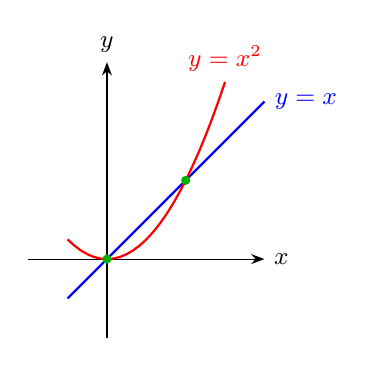
\begin{tikzpicture}
          \draw[->] (-1,0) -- (2,0) node[right]{$x$};
          \draw[->] (0,-1) -- (0,5/2) node[above]{$y$};
          \draw[blue,thick,domain=-1/2:2] plot (\x, \x) node[right]{$y = x$};
          \draw[red,thick,domain=-1/2:3/2] plot (\x, {\x*\x}) node[above]{$y =
          x^2$};
          \filldraw[green!70!black] (0,0) circle[radius=.5mm];
          \filldraw[green!70!black] (1,1) circle[radius=.5mm];
        \end{tikzpicture}
      \end{center}
    \end{column}
    \begin{column}{.45\textwidth}
      Now consider, for example, $g(x) = x^2$ on $[0,1]$.
      \vskip \baselineskip
      We can easily verify that $g(x) \in [0,1]$ for all $x \in [0,1]$.
      However, as can be seen from the figure on the left, $g$ has \emph{two}
      fixed points in $[0,1]$.
      \vskip \baselineskip
      To solve equation \eqref{eq:root-eq} via equation \eqref{eq:fp-eq}, we
      would rather have a \emph{unique solution}\footnote{To see why we want a
      unique solution, see slides \textcolor{green!70!black}{insert slide
      numbers}.} and therefore a unique fixed point.
    \end{column}
  \end{columns}
\end{frame}

\begin{frame}{Fixed Points}{Existence and uniqueness}
  Let us now determine the circumstances under which a fixed point of $g$ would
  be unique.
\end{frame}

\begin{frame}{Fixed Points}{Existence and uniqueness}
  We have proved the following
  \begin{theorem}[Uniqueness of a fixed point]
    Let $g : [a,b] \to \mathbb{R}$ be continuous on $[a,b]$ and $g(x) \in [a,b]$
    for all $x \in [a,b]$.
    If $g'$ exists on $(a,b)$ and there exists a constant $L \in (0,1)$ such
    that
    \[
      \abs{g'(x)} \leq L,\ \text{for all}\ x \in (a,b),
    \]
    then the fixed point $x^*$ of $g$ in $[a,b]$ is unique.
  \end{theorem}
\end{frame}

\section{Fixed Point Iteration}
\begin{frame}{Fixed Point Iteration}
  \label{fr:fp-iter-def}
  Equation \eqref{eq:fp-eq} suggests the following iterative method:
  \begin{equation} \label{eq:fp-iter}
    x_{k+1} = g(x_k)
  \end{equation}
  We refer this numerical method as a \emph{fixed-point iteration}.

  Equation \eqref{eq:fp-iter} is also called a \emph{simple iteration} and the
  numbers $x_k$ of the sequence it generates are called
  \emph{iterates}\footnote{Simple iteration and iterates are more generally used
  for iterative methods and the elements of the sequences these method
  generate.}.
\end{frame}

\begin{frame}{Fixed Point Iteration}
  \begin{example}
    Find a root of $f(x) = \mathrm{e}^x - 2x - 1$ in $[1,2]$ using fixed-point
    iteration with initial value $x_0 = 1$.
  \end{example}
  Rewrite $f(x) = \mathrm{e}^x - 2x - 1 = 0$ as
  \[
    \mathrm{e}^x = 2x + 1
    \quad \implies \quad
    x = \ln(2x + 1)
    \quad \implies \quad
    g(x) = \ln(2x + 1)
  \]
  \begin{center}
    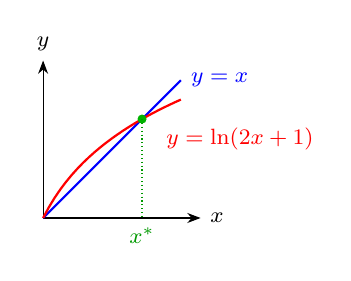
\begin{tikzpicture}[every node/.style={font=\footnotesize}]
      \draw[->] (0,0) -- (2,0) node[right]{$x$};
      \draw[->] (0,0) -- (0,2) node[above]{$y$};
      \draw[blue,thick,domain=0:7/4] plot(\x, \x) node[right]{$y = x$};
      \draw[red,thick,domain=0:7/4] plot(\x, {(ln(2*\x + 1)});
      \filldraw[green!70!black] (1.256431,1.256431) circle[radius=.5mm];
      \draw[green!60!black,densely dotted] (1.256431,1.256431) -- (1.256431,0)
      node[below]{$x^*$};
      \node at (2.5,1.0)[red]{$y = \ln(2x + 1)$};
    \end{tikzpicture}
  \end{center}
\end{frame}

\begin{frame}{Fixed Point Iteration}{Example (continued)}
  Using the initial value $x_0 = 1.0$, we obtain for the first five iterations
  \begin{align*}
    x_1 &= g(x_0) \approx 1.0986, &
    \abs{x_1 - x_0} &\approx 0.0986 \\
    x_2 &= g(x_1) \approx 1.1623, &
    \abs{x_2 - x_1} &\approx 0.0637 \\
    x_3 &= g(x_2) \approx 1.2014, &
    \abs{x_3 - x_2} &\approx 0.0391 \\
    x_4 &= g(x_3) \approx 1.2381, &
    \abs{x_4 - x_3} &\approx 0.0232 \\
    x_5 &= g(x_4) \approx 1.2460, &
    \abs{x_5 - x_4} &\approx 0.0136
  \end{align*}
  Since a tolerance was not specified in the problem statement, we can either
  stop here or continue with the iteration until we meet our own specified
  tolerance.

  To calculate the root to within a tolerance of $10^{-15}$ (the most accurate
  we can do on an average laptop) will take 58 iterations.
\end{frame}

\begin{frame}{Fixed Point Iteration}{Potential difficulty}
  One of the difficulties with fixed-point iteration is that there are
  potentially multiple ways of constructing $g$ from $f$.

  The following is taken from \cite[p.83]{atkinson1993elementary}.
  Consider solving the equation $x^2 - 5$ for the root $x^* = \sqrt{5}$.
  There are four possible fixed-point iteration formulae that may be used to
  solve this equation:
  \begin{align*}
    x_{k+1} &= g_1(x_k) = 5 + x_k - x_k^2, &
    x_{k+1} &= g_2(x_k) = \frac{5}{x_k}, \\
    x_{k+1} &= g_3(x_k) = 1 + x_k - \frac{x_k^2}{5}, &
    x_{k+1} &= g_4(x_k) = \frac{1}{2}\left(x_k + \frac{5}{x_k}\right).
  \end{align*}
\end{frame}

\begin{frame}{Fixed Point Iteration}{Why use fixed-point iteration?}
  Advantages:
  \begin{itemize}
    \item Fixed-point iteration \eqref{eq:fp-iter} is easier to calculate and
      implement\footnote{As compared to the bisection method.} (provided we know
      what $g$ is).
    \item Analysis for existence, uniqueness, and convergence behaviour is more
      simple than other root-finding methods.
  \end{itemize}
  Disadvantages:
  \begin{itemize}
    \item Convergence to a solution is not guaranteed\footnote{Although, we can
      determine for which $x$-values a problem may converge.}
    \item Construction of $g$ may prove difficult\footnote{Or potentially have
      other unwanted side-effects.}.
  \end{itemize}
\end{frame}

\section{Analysis}
\begin{frame}{Fixed Point Iteration}{Convergence analysis}
  The questions we now wish to answer are:
  \begin{itemize}
    \item Under which conditions does a solution for the fixed-point iteration
      \eqref{eq:fp-iter} exist?
    \item If such a solution exists, under which conditions will be unique?
  \end{itemize}
\end{frame}

\begin{frame}{Fixed Point Iteration}{Convergence analysis}
  To answer the first question, it suffices to show that
  \begin{equation} \label{eq:fp-limit}
    \lim_{k\to \infty} x_k = x^*,
  \end{equation}
  where $x_k = g(x_{k-1})$.

  To prove \eqref{eq:fp-limit}, we consider the absolut error $\abs{x_k - x^*}$.
  Recall that if $x^*$ is a root of $f$, then it is a fixed point of $g$.
  Now rewrite $\abs{x_k - x^*}$ as
  \[
    \abs{x_k - x^*}
    = \abs{g(x_{k-1}) - g(x^*)}.
  \]

\end{frame}

\begin{frame}{Fixed Point Iteration}{Convergence analysis}
  By the mean value theorem, there exists $\xi_{k-1} \in (a,b)$ such that
  \[
    g(x_{k-1}) - g(x^*) = g'(\xi_{k-1})(x_{k-1} - x^*)
  \]
  and, therefore,
  \[
    \abs{x_k - x^*}
    = \abs{g(x_{k-1}) - g(x^*)}
    = \abs*{g'(\xi_{k-1})}\,\abs{x_{k-1} - x^*}
  \]
\end{frame}

\begin{frame}{Fixed Point Iteration}{Convergence analysis}
  If we now assume that $\abs*{g'(x)} \leq L$, where $L \in (0,1)$, for all $x
  \in (a,b)$, then
  \[
    \abs{x_k - x^*}
    = \abs{g(x_{k-1}) - g(x^*)}
    = \abs*{g'(\xi_{k-1})}\,\abs{x_{k-1} - x^*}
    \leq L\abs{x_{k-1} - x^*}.
  \]
  Hence,
  \[
    \abs{x_k - x^*} \leq L\abs{x_{k-1} - x^*}.
  \]
  Applying this inequality inductively yields
  \[
    \abs{x_k - x^*} \leq L\abs{x_{k-1} - x^*}
    \leq L^2\abs{x_{k-2} - x^*}
    \leq \dotsb
    \leq L^k\abs{x_0 - x^*}
  \]
\end{frame}

\begin{frame}{Fixed Point Iteration}{Convergence analysis}
  Since $0 < L < 1$, it follows that
  \[
    \lim_{k\to\infty} L^k = 0
  \]
  and, therefore,
  \[
    \lim_{k\to\infty}\abs{x_k - x^*} \leq \lim_{k\to\infty} L^k\abs{x_0 - x^*}
    = 0.
  \]
  Since $\lim_{k\to\infty} 0 \leq \lim_{k\to\infty}\abs{x_k - x^*}$, by the
  squeeze theorem then follows that
  \[
    \lim_{k\to\infty} \abs{x_k - x^*} = 0
  \]
  and, therefore,
  \[
    \lim_{k\to\infty} x_k = x^*.
  \]
\end{frame}

\begin{frame}{Fixed Point Iteration}{Convergence analysis}
  We have just proved the following
  \begin{theorem}[Fixed-Point Theorem]
    Let $g : [a,b] \to \mathbb{R}$ be continuous on $[a,b]$ and $g(x) \in [a,b]$
    for all $x \in [a,b]$.
    Suppose that $g'$ exists on $(a,b)$ and $L \in (0,1)$ exists such that
    \[
      \abs{g'(x)} \leq L,
      \quad\text{for all}\ x \in [a,b].
    \]
    Then, for any number $x_0 \in [a,b]$, the sequence defined by
    \[
      x_{k+1} = g(x_k), \quad k \in \mathbb{N},
    \]
    converges to the unique fixed point $x^* \in [a,b]$.
  \end{theorem}
\end{frame}

\begin{frame}{Questions To Ponder}
  \begin{itemize}
    \item   
  \end{itemize}
\end{frame}

\section{Exercises}
\begin{frame}{Exercises}
\end{frame}

\begin{frame}{Exercises}
\end{frame}


\begin{frame}{Further Reading}
  \nocite{burden2015numerical,hamming1986numerical,isaacson1994analysis,suli2003introduction,gerald2004applied,atkinson1993elementary}
  \printbibliography
\end{frame}

\appendix
\begin{frame}{Fixed Points}{Behaviour of fixed points}
\end{frame}

\end{document}
